%!TEX = xelatex
\documentclass[a4paper]{article}
\usepackage[margin=1in]{geometry}
\usepackage{graphicx}
\usepackage{amsmath}
\usepackage{amssymb}
\usepackage{xcolor}
    \newcommand{\todo}[1]{\textcolor{red}{[ #1 ]}}
    \newcommand{\instruction}[1]{\textcolor{orange}{#1}}
    % \renewcommand{\todo}[1]{} % Uncomment to hide todos.
    % \renewcommand{\instruction}[1]{} % Uncomment to hide instructions.

\newcommand{\hidden}[1]{}

\usepackage{biblatex}
    \addbibresource{references.bib}

\usepackage[colorlinks=false]{hyperref}

\title{STATS 402 - Interdisciplinary Data Analysis\\
    Resource-Constrained Deep Reinforcement Learning for Battlesnake\\
    Milestone Report: Stage 2
}
\author{Steven Hé (Sīchàng)\\
    sichang.he@dukekunshan.edu.cn
}

\begin{document}
\maketitle

\instruction{
    There are no specific requirements for the stage 2 report since the progress may vary among different groups. Generally, there are four parts you need to cover in your report.
}

\subparagraph{Abstract}

Placeholder~\cite{battlesnake}.

\section{Current Status}

\todo{The current status of your project.\\
    For example, the detailed techniques you adopted to conduct the project. Has your group made any technical route adjustments? This part is essential for the groups whose actual adopted method is different from their milestone report 1. You need to explain the reason for the change.
}

\subsection{Technical Route Adjustments}

Although we planned to use the Gymnasium environment
library~\cite{farama2024gymnasium} in the proposal~\cite{proposal},
we found that it does not support multi-agent environments like the ones we have
in Battlesnake. Therefore,
we adjusted the environment library choice to be
Pettingzoo~\cite{terry2021pettingzoo} instead.
Pettingzoo supports simultaneous-move multi-agent environments via its Parallel
API\footnote{\url{https://pettingzoo.farama.org/api/parallel/}},
and can be made compatible with Stable Baselines3~\cite{raffin2024stable}
using SuperSuit~\cite{SuperSuit}.

\subsection{Feature Extraction Implementation }

The Pettingzoo environment has been implemented based on the feature extraction
described in the
proposal\footnote{\url{https://github.com/SichangHe/STATS402_course_project/tree/main/battlesnake_train/battlesnake_gym}}.
This environment has been wrapped using SuperSuit and tested against Stable
Baselines3 APIs,
and appears to be working properly as a Stable Baselines3 environment in our API
unit testing.

Game simulation is powered by the implementation in~\cite{wrenger2024rusty},
which leads to two challenges. First, the game simulation is written in Rust,
while the Pettingzoo environment needs to be in Python. To bridge this gap,
we leverage a mature Rust-Python interoperability solution,
the PyO3 library~\cite{pyo3} and the build tool Maturin~\cite{maturin}.
A wrapper Rust struct is created and registered as a Python class to represent a
Battlesnake game,
and provide methods for the Pettingzoo environment to interact with.
Another Python class (\textsf{BattlesnakeEnv})
then wraps the Rust struct and implements the Pettingzoo Parallel API. Second,
the game simulation only presents the original board state,
without any transformations based on each snake agent's position or orientation
like we had planned. Therefore,
we referred to the feature extraction implementation
in~\cite{siddiqui2020multiagent},
and reimplemented our similar approach in Rust.

To be more specific,
the feature matrix of $\mathbb R^{9\times21\times21}$ is constructed in Rust and
converted into a Numpy array~\cite{harris2020array}
to suit the methods in \textsf{BattlesnakeEnv}. Notably,
the features are nine layers instead of ten,
as incorrectly stated in the proposal; layer 0 represents walls,
layers 1 represents the agent's body, layer 2, 4,
6 represent the head of each opponent snake, layer 3, 5,
7 represent the body of each opponent snake, and layer 8 represents food.
To implement our proposed feature extraction,
we first construct three intermediate values:
each snake's body layer on the original board,
the order of the snakes based on their length and health,
and the head values of ordered opponent snakes from each snake's perspective.
We then calculate the full feature matrix for each snake's observation without
the rotation, and the facing of each snake. Finally,
these two values are sent to Python,
where we conveniently construct the final feature matrix by rotating the feature
matrix in Numpy according to the snake's facing. In this process,
a large number of indexing is used to construct the feature matrix,
causing difficulties to debug. Though,
we tested the implementation by inspecting the intermediate values,
confirming its correctness.

Besides feature extraction,
the Rust implementation also converts relative actions input from the Python
side into absolute actions for the game simulation. For example,
if an agent's head is facing ``left'' and the relative action they output is
``right'',
our implementation converts the action to ``up'' before sending it to the game
simulation.
This facing detection is based on the relative position of the agent's head and
second body part. The four orientations ``up'', ``right'', ``down'',
and ``left'' are represented as integers 0, 1, 2, 3, respectively,
in a clockwise order.
Both the action input $A_{relative}$ and the facing detection $F$ use this representation,
so the absolute action $A_{absolute}=(A_{relative}+F)\bmod 4$,
and the facing can be directly used for the rotation in Numpy mentioned above.

\section{Data Preprocessing}

\todo{Demonstrate some initial data preprocessing results if you have.}

We tested the environment with the built-in multilayer perceptron (MLP)
policy from Stable Baselines3~\cite{raffin2024stable}.
For both the actor and the critic,
the MLP has two hidden layers of size 64 with ReLU activation.
Training the model on an M1 MacBook for 1,000,000 steps took 8 minutes 37
seconds, while leveraging most of the CPU cores.

The initial training results were suspicious. For example,
as shown in Fig.~\ref{fig:render},
the agents controlled by the MLP model are not even able to avoid colliding with
the walls. Looking into several outputs of \textsf{step}
method calls on the wrapped environment, we discovered that the \textsf{done}
fields are always \textsf{False}, raising suspicions that the environment was
not working properly after the wrapping with SuperSuit~\cite{SuperSuit}.

\begin{figure}
    \centering
    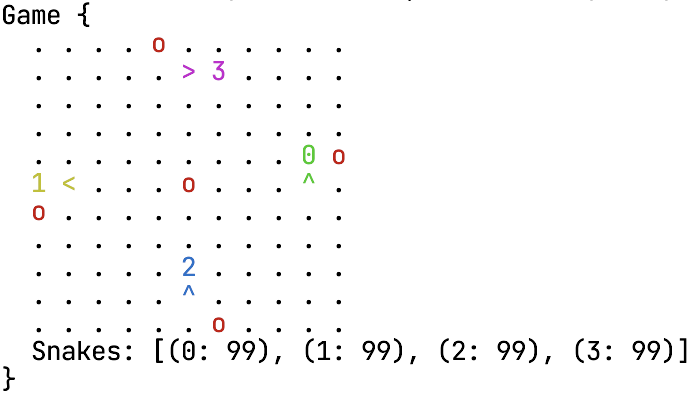
\includegraphics[width=0.4\linewidth]{game_render_eg.png}\quad
    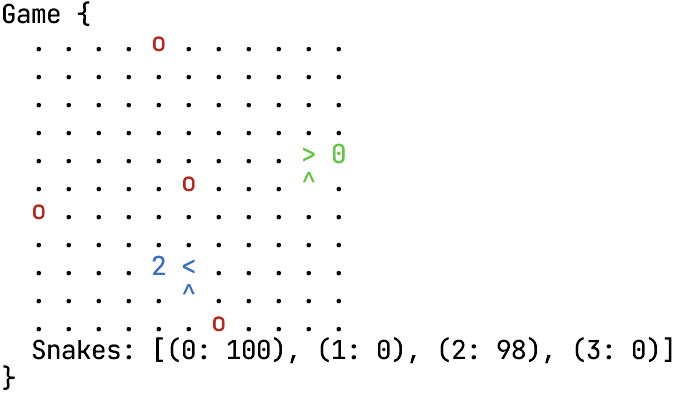
\includegraphics[width=0.4\linewidth]{game_render_eg1.png}
    \caption{ANSI rendering of the game simulation for debugging purposes.
        The right figure shows state of the game board after each snake in the
        left figure took an action.
    }
    \label{fig:render}
\end{figure}

After removing entirely the rewards and other parameters for the dead agents,
the results are much more reasonable. Based on manual inspection,
the agents are now able to avoid walls,
interestingly by circling the grid in a counter-clockwise manner, as demonstrated in Fig.~\ref{fig:render2}. However,
they still do not seem to be able to avoid colliding with each other.
The agents also seem to be agnostic about food,
which is likely due to the lack of direct rewards for eating food.
Overall, the fact that the agents are able to avoid walls is promising,
indicating that they should be able to learn more complex strategies with
a more sophisticated model.

\begin{figure}
    \centering
    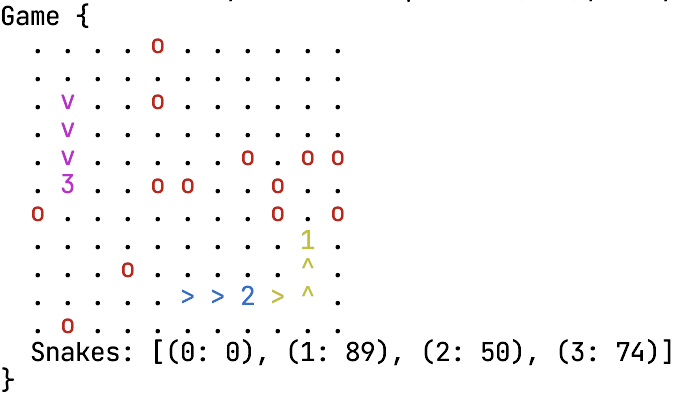
\includegraphics[width=0.4\linewidth]{game_render_eg2.png}\quad
    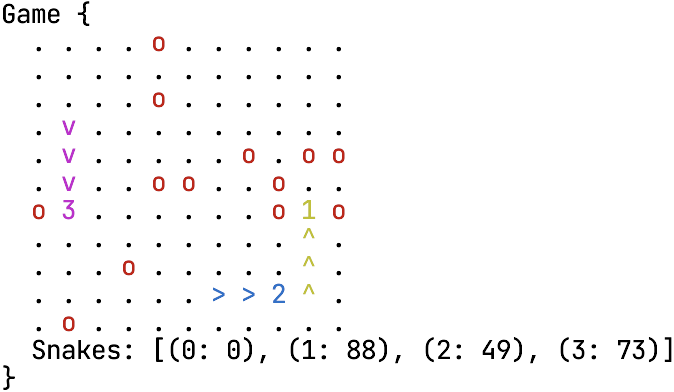
\includegraphics[width=0.4\linewidth]{game_render_eg3.png}
    \caption{ANSI rendering of the game simulation after removing return values
        for dead agents. The right figure is one step after the left figure.
    }
    \label{fig:render2}
\end{figure}


\section{Plan for the Next Two Weeks}

\instruction{Maximum 6 pages}

\printbibliography

\end{document}
